\documentclass{standalone}

\usepackage{amssymb}
\usepackage{amsthm}
\usepackage{amsmath}


\usepackage{tikz}
\usetikzlibrary{shapes,backgrounds,calc,patterns}


\begin{document}
	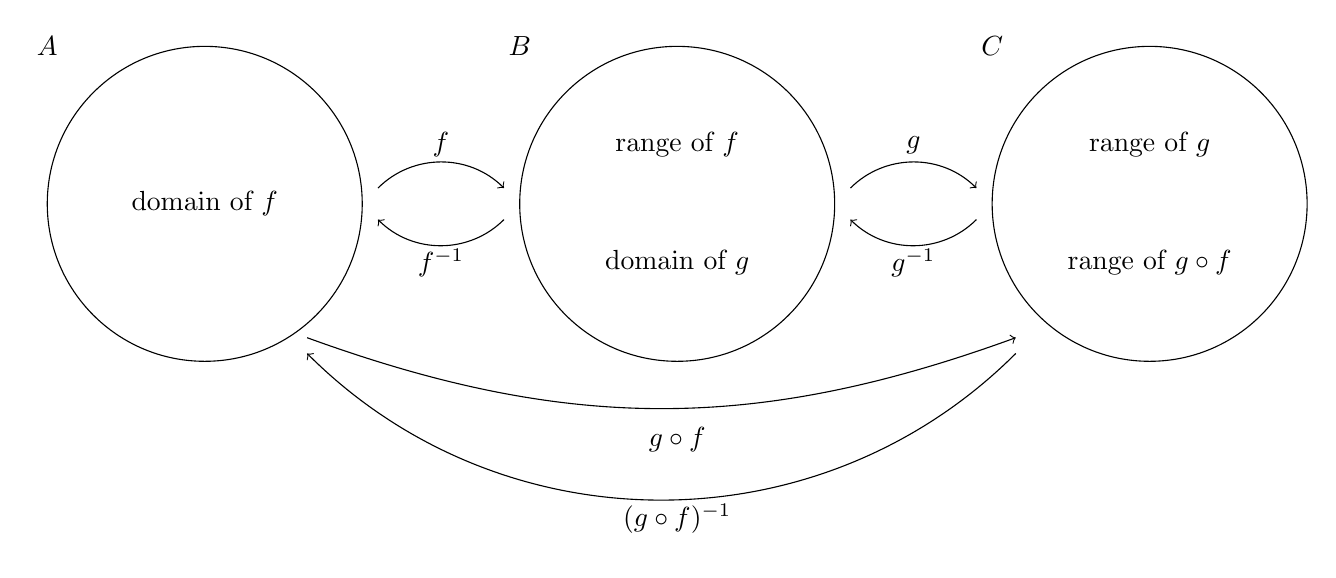
\begin{tikzpicture}
		\draw (-3,0) circle (2);
		\node at (-3,0) {domain of \(f\)};
		\node at (-5,2) {\(A\)};
		
		\draw (3,0) circle (2);
		\node at (3,.75) {range of \(f\)};
		\node at (3,-.75) {domain of \(g\)};
		\node at (1,2) {\(B\)};	
		


		
		\draw[->] (-.8,.2) to[out=45,in=135] (.8,.2);
		\node at (0,.75) {\(f\)};
		\draw[->] (.8,-.2) to[out=225,in=-45] (-.8,-.2);
		\node at (0,-.75) {\(f^{-1}\)};
		
		
		\draw (9,0) circle (2);
		\node at (7,2) {\(C\)};	
		\node at (9,.75) {range of \(g\)};
		\node at (9,-.75) {range of \(g\circ f\)};	
		
		\draw[->] (5.2,.2) to[out=45,in=135] (6.8,.2);
		\node at (6,.75) {\(g\)};
		\draw[->] (6.8,-.2) to[out=225,in=-45] (5.2,-.2);
		\node at (6,-.75) {\(g^{-1}\)};
		
		\draw[->] (-1.7,-1.7) to[out=-20,in=200] (7.3,-1.7);
		\node at (3,-3) {\(g\circ f\)};	
		
		\draw[->] (7.3,-1.9) to[out=225,in=-45] (-1.7,-1.9);
		\node at (3,-4) {\((g\circ f)^{-1}\)};	
	\end{tikzpicture}
	
	
	
\end{document}